\documentclass{article}
\usepackage{amsmath}
\usepackage{graphicx}
\title{Results}

\author
{
    Dereck Piché \and
    Guillermo Martinez \and
    Jonas Gabirot \and
}

\begin{document}
\maketitle

\section{Results}

\subsection{Baseline: XGB}
We trained and tested an Extreme Gradient Boosting (XGB) regressor using DNA sequences as features and their respective free-energy levels as labels. 900 000 samples were used for training and 100 000 samples for testing. The model's train and test performance were assessed by calculating the Mean Square Error (MSE) between the predicted and actual free energy levels given specific DNA sequences. 0.993166 and 1.016363 MSE were achieved on train and test evaluation respectively. These results will be used as baselines to evaluate further models' predictive performance.


\subsection{Baseline: MLP}

\begin{figure} \label{fig:template}
    \caption{Voici le template} \center
    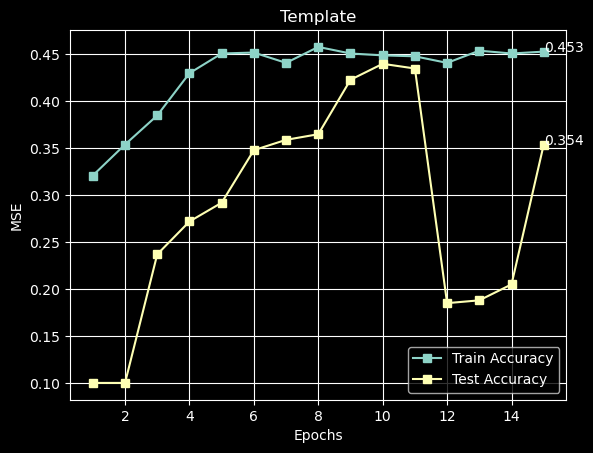
\includegraphics[width=0.7\textwidth]{images/2023-03-28-10-29-38.png}
\end{figure}

\subsection{LSTM}

\subsection{Regression Transformer}
We built a model using the main components of the Transfomer architecture proposed in \cite{transformers} for our regression task. Our regression transformer is made up of a sequence of encoder layers. Each of the encoder layers contains 8 attention heads with a ReLU activated linear layer. We trained the transformer on $9 ,000, 000$ DNA sequences of length $30$ and tested it's MSE loss on the remaining $100,000$ training examples. The transformer used the same positionnal encoding as the one proposed in \cite{transformers}. The DNA sequences came in string form. Each of the 4 tokens were transformed into an integer and fed into a learned embedding layer that transformed them into vectors of 16 dimensions. The number of dimensions of the embeddings is a bit arbitrary, but since it works really well we left it there. The accuracy troughout the epochs can be seen in figure \ref{fig:transformer_accuracy}. 

\begin{figure} \label{fig:transformer_accuracy}
    \caption{Voici le template} \center
    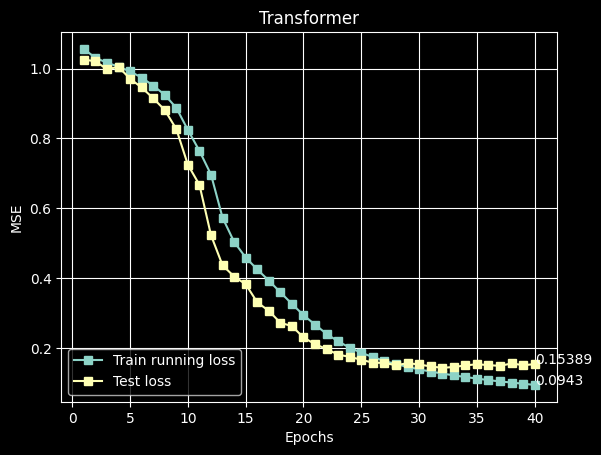
\includegraphics[width=0.7\textwidth]{images/2023-04-02-13-48-49.png}
\end{figure}

\section{Analysis}


\subsection{Comparisons}

\section{Conclusion}

\bibliography{bibliography}
\bibliographystyle{plain}
\end{document}
